\documentclass[11pt]{article}

%\usepackage[nosol]{optional}
\usepackage[sol]{optional}

\usepackage {tikz}
    \usetikzlibrary{calc,shapes,arrows,automata,positioning,cd}
    \tikzset{
     dot node/.style={font=\sffamily\small},
      cfgedge/.style   = {black, ->, >=stealth},
      forward/.style = { blue, ->, >=angle 45},
      backward/.style = { red, densely dashed, ->, >=latex' },
      backwardleft/.style = { red, densely dashed, <-, >=latex' },
      position/.style args={#1:#2 from #3}{
        at=(#3.#1), anchor=#1+180, shift=(#1:#2)
    },
    }
    \usepackage{xcolor}

\usepackage{listings, ../listings-rust/listings-rust}
\usepackage{listings}
\usepackage{xcolor}
\definecolor{codegreen}{rgb}{0,0.6,0}
\definecolor{codegray}{rgb}{0.5,0.5,0.5}
\definecolor{codepurple}{rgb}{0.58,0,0.82}
\definecolor{backcolour}{rgb}{0.95,0.95,0.92}
\lstset{
    language=Python,
    keepspaces=true,
    numbers=left,
    backgroundcolor=\color{backcolour},
    commentstyle=\color{codegreen},
    basicstyle=\ttfamily,
    otherkeywords={self,True,False,yield},
    keywordstyle=\ttfamily\color{blue!90!black},
    %basicstyle=\footnotesize,
    keywords=[3]{ttk},
    keywordstyle={[2]\ttfamily\color{orange!80!orange}},
    keywordstyle={[3]\ttfamily\color{red!80!orange}},
    emph={MyClass,__init__},
    emphstyle=\ttfamily\color{red!80!black},
    stringstyle=\color{green!80!black},
    showstringspaces=false
}

\newcommand{\N}{\mathbb{N}}
\newcommand{\Z}{\mathbb{Z}}

% For proof.
\usepackage{amsmath,amsthm,amssymb}

\usepackage{enumerate}
\usepackage{graphicx}
\usepackage{float}
\usepackage{subcaption}
\usepackage{comment}

\renewcommand{\topfraction}{.9}
\renewcommand{\textfraction}{.1}

\usepackage{fullpage,amsmath,amssymb}
\usepackage[colorlinks=true,citecolor=blue,linkcolor=blue]{hyperref} % for href links, and also makes \ref and \eqref clickable in the PDF

% parenthetical comment to state verbally but not write on the board
\newcommand{\com}[1]{\footnote{#1}}

\newcommand{\deltahat}{\widehat{\delta}}

\newcommand{\QuasiP}{\mathsf{QuasiP}}

\newcommand{\TIME}{\mathsf{TIME}}

\usepackage{fancyhdr}
\fancypagestyle{firststyle}
{
    \fancyhf{}
    \fancyhead[C]{Copyright \copyright\ \today, David Doty}
}


\title{Homework 5 \opt{sol}{Solutions} -- ECS 220, Winter 2020}
\date{}
\begin{document}
\maketitle
\thispagestyle{firststyle}
\vspace{-2.0cm}

\section{Alphabetic Geography. (Textbook problem 8.20)}
\begin{quote}
    In traditional Geography, a move from a city $u$ to a city $v$ is allowed if $v$ starts with the same letter that $u$ ends with.
    Let’s say that a directed graph $G$ is \emph{alphabetic} if it of this form:
    in other words, if for some finite alphabet $A$,
    each vertex $u$ can be assigned a pair $f(u)$, $\ell(u) \in A$
    such that there is an edge from $u$ to $v$
    if and only if $\ell(u) = f(v)$.
    Give a small example of a graph that is not alphabetic.
    Then show that \textsc{Alphabetic-Geography} is $\mathsf{PSPACE}$-complete,
    by converting any graph to an alphabetic one
    (albeit with an alphabet that grows with the number of vertices).
\end{quote}
The last sentence is asking for a \emph{reduction} from $\textsc{Geography}$ to $\textsc{Alphabetic-Geography}$:
convert any graph $G$ into an alphabetic graph $G_\alpha$ such that
Player 1 has a winning strategy on $G$
if and only if
Player 1 has a winning strategy on $G_\alpha$.

\section{solution}
\subsection*{Non-alphabetic graph}

\begin{figure}[h]
    \centering
    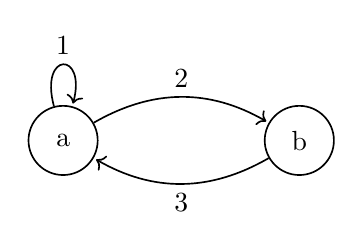
\begin{tikzpicture}[shorten >=1pt,node distance=3cm,on grid,auto, semithick]
        \node [state] (a)               {a};
        \node [state] (b) [right of=a]  {b};

        \path[->]
        (a) edge [loop above] node {1} ()
        (a) edge [bend left] node {2} (b)
        (b) edge [bend left] node {3} (a);
    \end{tikzpicture}
    \caption{A graph that is not alphabetic}
\end{figure}

This graph is not alphabetic.
As it clearly shows that $l(a) = f(a)$(edge 1), $l(a) = f(b)$(edge 2), $l(b) = f(a)$(edge 3).
Therefore we have $l(b) = f(b)$, indicating that there should also be a self-loop over $b$, but there isn't.

\subsection*{Proof of $\mathsf{PSPACE}$-complete}
As the problem description mentioned, the significant step to show \textsc{Alphabetic-Geography} is $\mathsf{PSPACE}$-complete is to convert any graph to an alphabetic one. The difficulty is that some given graph may not be alphabetic, that is we have no methods to assign $f(u)$ and $l(u)$ to make the whole graph has no contradictions. Here we provide a method to do the conversion from any arbitrary graph:\\
Suppose the finite alphabet called $\Sigma$ (same as Exercise d.), $|\Sigma|=k$ and each elements in $\Sigma$ is $\sigma_i, i\in \{1,2,...,k\}$,\\
\color{red} For each edge $e=(u,v)$ in the origin graph $G$, we insert two nodes $x,y$ onto the edge in graph $G_\alpha$.\color{black}\\
That makes the origin directed edge $e=(u,v)$ becomes $(u,x),(x,y),(y,v)$. \\
Then we do the alphabetic-assignment. For each edge in the origin graph like $e=(u,v)$, we make $f(x)=l(u), l(y)=f(v)$, and assign $l(x)=f(y)$ with $\sigma_i$ that never assigned before. To show how it works, we use a simple graph shown below to express the process of assignment:
\begin{figure}[h]
    \centering
    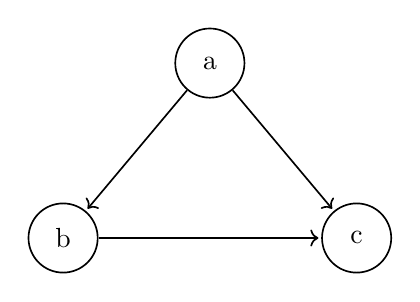
\begin{tikzpicture}[shorten >=1pt,node distance=3cm,on grid,auto, semithick]
        \node [state] (a)   {a};
        \node [state] (b) [position=230: 2cm from a]  {b};
        \node [state] (c) [position=310: 2cm from a]  {c};
        \path[->]
        (a) edge (b)
        (a) edge (c)
        (b) edge (c);
    \end{tikzpicture}
    \caption{Origin graph $G$}
\end{figure}

\begin{figure}[h]
    \centering
    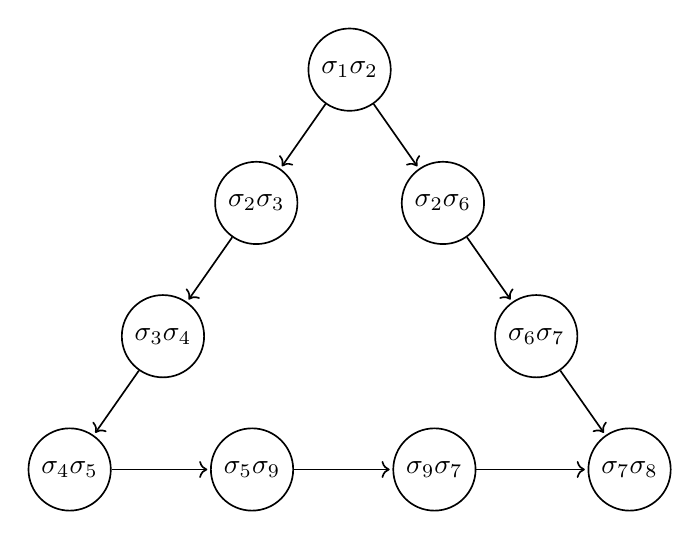
\begin{tikzpicture}[shorten >=1pt,node distance=3cm,on grid,auto, semithick]
        \node [state] (a)   {$\sigma_1\sigma_2$};
        \node [state] (b) [position=235: 1cm from a]  {$\sigma_2\sigma_3$};
        \node [state] (c) [position=235: 1cm from b]  {$\sigma_3\sigma_4$};
        \node [state] (d) [position=235: 1cm from c]  {$\sigma_4\sigma_5$};
        \node [state] (e) [position=305: 1cm from a]  {$\sigma_2\sigma_6$};
        \node [state] (f) [position=305: 1cm from e]  {$\sigma_6\sigma_7$};
        \node [state] (g) [position=305: 1cm from f]  {$\sigma_7\sigma_8$};
        \node [state] (h) [position=0: 1.25cm from d]  {$\sigma_5\sigma_9$};
        \node [state] (i) [position=0: 1.25cm from h]  {$\sigma_9\sigma_7$};
        \path[->]
        (a) edge (b)
        (b) edge (c)
        (c) edge (d)
        (a) edge (e)
        (e) edge (f)
        (f) edge (g)
        (d) edge (h)
        (h) edge (i)
        (i) edge (g);
    \end{tikzpicture}
    \caption{The alphabetic-assignment $G_\alpha$}
\end{figure}
    Then we prove that Player 1 has a winning strategy on $G$ if and only if Player 1 has a winning strategy on $G_\alpha$. Here we can see that the reason why we insert \color{red} 2 \color{black} nodes onto an edge is that it won't affect the nodes that two players will choose in the origin graph $G$, since the two inserted nodes make it one directional path. Also, these intermediate points won't be the start point since the start point will always be the corresponding node in origin graph $G$. So that Player 1 has a winning strategy beginning at point $v$ if and only if he has a winning strategy beginning at the corresponding point in $G_\alpha$.

\end{document}